\documentclass[10pt,journal]{IEEEtran}

\usepackage{amsmath}
\usepackage{amssymb}
\usepackage{booktabs}
\usepackage{graphicx}
\usepackage{hyperref}
\usepackage[section]{placeins}

\title{Pre-generation State Structures under Multimodal Affective Conflict and Their Association with Affective Misreads}
\author{Haonan Zhang}

\begin{document}
\maketitle

\begin{abstract}
Multimodal affective cues do not always point in the same direction, yet an
output-level correct/incorrect label alone cannot explain how a model internally
handles such conflict. We study how multimodal affective conflict is organized in
the model's internal state before the first generated token, and how these
pre-generation state structures are associated with subsequent affective misreads.
For each input, we register two unimodal conditions and their joint condition,
extract their complete layer trajectories at \(t_0\) under equivalent prompts, and
learn their ordered relation with a Trajectory Manifold Encoder (TME) supervised
only by Conflict/Aligned labels. We then characterize the frozen condition states
along three complementary coordinates: State Dispersion, which measures prompt
sensitivity; Modality Split, which measures separation between unimodal states; and
signed Joint Lean, which measures the direction of the joint state. Calibrated
thresholds organize these coordinates into four descriptive State Patterns:
Confusion, Consensus, Balanced, and Dominant. These coordinates are not combined
into a universal misread score, and the patterns are not an error taxonomy. Our
evaluation separates Conflict/Aligned structure from a controlled, Conflict-only
analysis of associations with Misread outcomes, and compares complete frozen
representations under matched data, supervision budgets, probes, and test sets. This
formulation turns affective misreading from a single endpoint into an interpretable
sequence from input conflict, through pre-generation state structure, to subsequent
behavior and response-level mitigation.
\end{abstract}

\section{Introduction}

Multimodal models increasingly interpret people from several affective channels at
once. In favorable cases, facial behavior, language, and voice reinforce one another.
In harder cases, a positive utterance may accompany visible strain, or a calm face may
co-occur with distressed speech. Such conflict matters because a model can produce a
fluent response while grounding its affective interpretation in the wrong cue. An
output-level label tells us whether this affective misread occurred, but not what
internal configuration preceded it. Multimodal affect datasets such as CH-SIMS v2
provide a basis for studying how these cues interact \cite{liu2022chsims}; our concern
is the organization of that interaction inside a generative model before it speaks.
Recent conflict-centered benchmarks show systematic modality bias and performance
degradation under affective conflict \cite{han2025benchmarking,sun2026emomm}, but
output accuracy and attention summaries do not by themselves describe the geometry
of the complete pre-generation relation.

We therefore ask a two-part question: how is multimodal affective conflict organized
in the model's internal state before the first generated token, and how are these
pre-generation state structures associated with subsequent affective misreads? This
question differs from moving a binary error classifier to an earlier time step. It
also differs from learning another Conflict detector. Conflict/Aligned describes a
property of the registered multimodal input, whereas Misread/Non-misread describes a
model's later behavior relative to a reference affect description. We use the former
to learn a stable relation space and reserve the latter for an independent behavioral
analysis. Misread labels are never used to train the state encoder.

Our measurement point is \(t_0\), the last conditioning state before the first
generated token. For every sample, we construct two unimodal conditions \(M_1\) and
\(M_2\), together with the joint condition \(M_{12}\), and extract their complete
layer trajectories under \(P\) registered, semantically equivalent prompts. The
Trajectory Manifold Encoder (TME) maps each condition trajectory to a unit-sphere
embedding and maps the ordered three-condition relation to a sample-level relation
embedding. TME learns this relation from sample-level Conflict/Aligned supervision;
the class label is not copied onto any individual condition trajectory. After
training, the encoder is frozen. Its condition-level embeddings and sample-level
relation embeddings are cached separately because they answer different questions.

The condition-level embeddings define three complementary State Indices. State
Dispersion \(S\) asks whether the internal state remains stable when the same task is
phrased in equivalent ways. Modality Split \(D\) asks whether the two unimodal inputs
pull the model toward distinct internal directions. Signed Joint Lean \(R\) asks
which unimodal direction the joint input approaches; by convention, \(R>0\) denotes
V-lean and \(R<0\) denotes T/A-lean. Put simply, \(S\) asks whether the model stands
steadily, \(D\) asks whether the modalities pull apart, and \(R\) asks which way the
joint state leans. They are coordinates of different phenomena, not three versions of
one severity variable, and we do not combine them into a universal Misread
probability.

Aligned calibration data partition these coordinates into four State Patterns.
Confusion means that equivalent prompts move the state too much to assign a stable
direction. Among stable states, Consensus means that the unimodal states do not
separate significantly; Balanced means that they separate but the joint state does
not lean significantly toward either one; and Dominant means that a significant
split is accompanied by a significant directional lean. State Pattern is therefore
a mechanism-motivated descriptive partition of pre-generation configurations, not a
taxonomy of errors. A Confusion state may still yield a correct description, and a Dominant state
may lean toward either the reference-supported cue or a misleading surface cue.
Likewise, Consensus may reflect genuinely aligned evidence or a failure to encode an
objective conflict. The patterns describe how a model organizes evidence, not whether
its eventual answer must be right or wrong.

This distinction determines our evidence chain. First, we measure whether Conflict
inputs have a different prevalence of affective misreads from Aligned inputs. Second,
we test whether Conflict and Aligned inputs differ in their State Index and State
Pattern distributions. Third, within Conflict samples only, we measure how \(S\),
\(D\), State Pattern, and the direction of \(R\) are empirically associated with
Misread outcomes. Signed Joint Lean primarily explains direction; its absolute value
is not treated as a general error score. Fourth, we freeze each learned representation
and train the same controlled Conflict-only Misread probe to test how much behavioral
information the representation retains. Finally, we evaluate whether state-guided
responses reduce response-level Affective Misattribution by preserving overlooked
cues. This last step does not claim to change the base model's earlier Diagnostic
Misread.

Our representation comparison follows the same boundary. Single-Point,
Trajectory MLP, and TME use the same master split, Conflict/Aligned data, Conflict
supervision budget, three conditions, probe architecture, probe budget, and held-out
intersection. Each method nevertheless retains its native representation and training
objective: the two baselines use ordinary classifiers, whereas TME uses its spherical
ordered-relation module and Proxy Anchor objective. The comparison therefore concerns
each complete method. Without component ablations, an advantage cannot be assigned
solely to full-layer trajectories, the manifold geometry, or Proxy Anchor.

The contributions of this work are as follows:
\begin{itemize}
  \item We formulate affective conflict analysis as the measurement of
  pre-generation state structure and its association with subsequent Misread
  behavior, explicitly separating input-side Conflict/Aligned supervision from
  output-side Misread evaluation.
  \item We introduce TME and a registered three-condition, multi-prompt protocol that
  exports condition-level spherical states and sample-level relation embeddings at
  \(t_0\).
  \item We define State Dispersion, Modality Split, signed Joint Lean, and four
  calibrated State Patterns that explain complementary internal phenomena without
  constructing a scalar error score or an ordered error hierarchy.
  \item We establish a matched evaluation of complete frozen representations with a
  Conflict-only Misread probe, and separate this representation analysis from the
  downstream evaluation of response-level Affective Misattribution.
\end{itemize}

\section{Related Work}

\subsection{Multimodal Affective Understanding and Conflict}

Multimodal affect datasets such as CH-SIMS v2 provide the empirical basis for studying
how visual, textual, and acoustic cues jointly express sentiment \cite{liu2022chsims}.
CA-MER studies realistic audio--visual emotion conflicts and documents systematic
modality bias in multimodal emotion reasoning \cite{han2025benchmarking}. EmoMM
extends conflict-centered evaluation to aligned, conflict, and missing-modality
settings and analyzes model behavior under these conditions \cite{sun2026emomm}.
Most task formulations ultimately score an output label or description. Our focus is
instead the relation among two unimodal states and their joint state at \(t_0\) under
controlled Conflict and Aligned inputs. Conflict/Aligned is used as input-side
relation supervision; subsequent Misread behavior remains a separate outcome.

\subsection{Pre-generation State Analysis and Uncertainty}

Semantic uncertainty measures invariance in generated meanings
\cite{kuhn2024semanticuncertainty}. In contrast, our state is measured at \(t_0\) from
registered hidden-state trajectories, before any diagnostic description is generated.
HALP shows that pre-generation internal representations can support probes of later
hallucination outcomes \cite{kogilathota-etal-2026-halp}. This supports the broader
premise that subsequent behavior can be readable before decoding, but hallucination
is not affective Misread and our objective is not a detector. We characterize the
three-condition structure first and examine its behavioral association separately.
We do not turn the resulting coordinates into one uncertainty or Misread score.
State Dispersion, Modality Split, and signed Joint Lean describe prompt stability,
unimodal separation, and joint direction, respectively.

\subsection{Frozen Representation Evaluation}

Our learned representations are evaluated only after the Conflict/Aligned encoders
are frozen. A controlled MLP probe is trained and tested within Conflict samples to
measure association with later Misread labels. Single-Point, Trajectory MLP, and TME
share data, supervision budgets, probes, and test intersections, while retaining
their native representation structures and objectives. This evaluates each complete
method rather than attributing a difference to one unablated component.

\subsection{State-guided Response}

State-guided response is an application of state analysis rather than the central
claim. It is evaluated by response-level Affective Misattribution and cue preservation;
it is not presented as correcting the base model's earlier Diagnostic Misread.

\section{Methodology}

\subsection{Task Setup}

Samples are grouped as Conflict, Ambiguous, or Aligned.
The main experiments focus on Conflict and Aligned samples.
For each protocol, we construct \(M_1\), \(M_2\), and \(M_{12}\) conditions.

\begin{figure}[t]
  \centering
  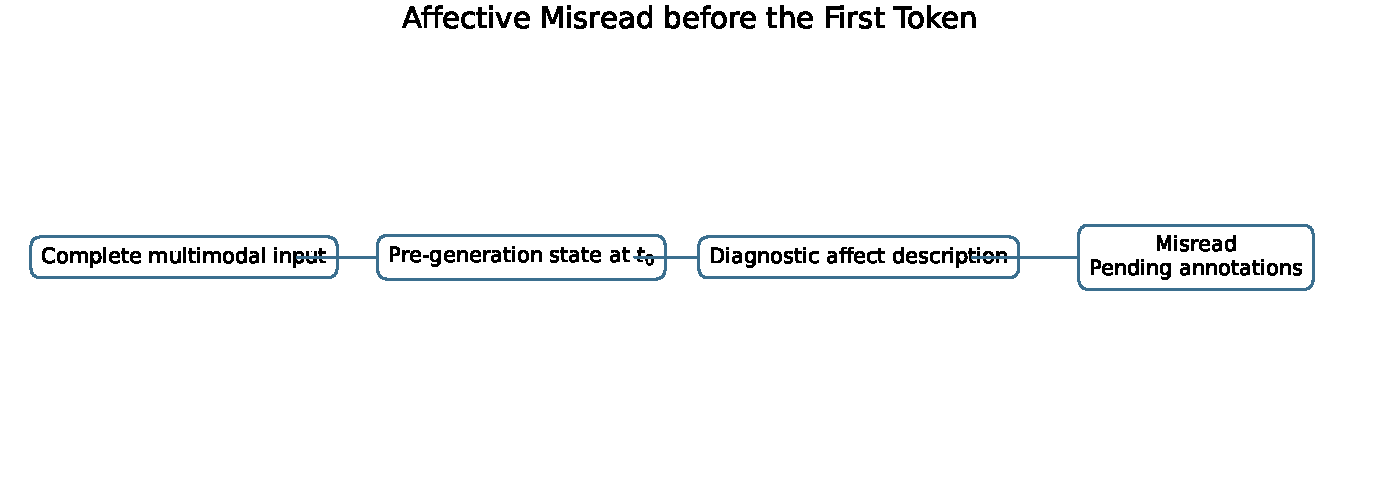
\includegraphics[width=\linewidth]{figures/generated/fig01_problem_protocol.pdf}
  \caption{Affective Misread before the first token.}
  \label{fig:problem-protocol}
\end{figure}

\subsection{Pre-generation State Extraction at \(t_0\)}

\(t_0\) is the last conditioning state before the first generated token.
The extraction uses prefill hidden states and can reuse prompt-side computation when supported.

\subsection{Pre-generation Trajectory Representation}

The state object is a full-layer prefill trajectory rather than a single hidden-state point.
The trajectory encoder maps this object into a manifold-aware representation space.

\begin{figure}[t]
  \centering
  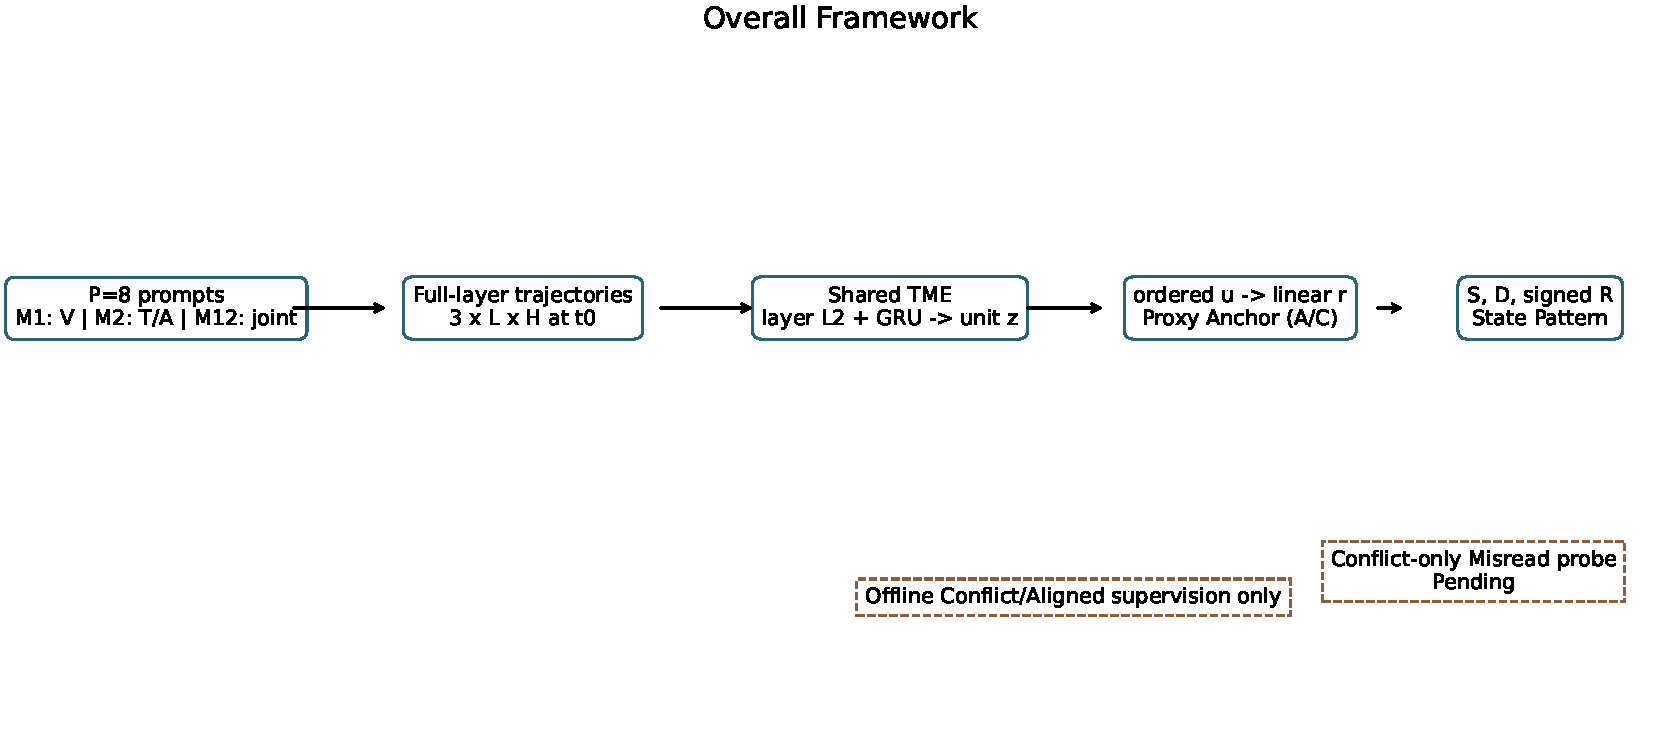
\includegraphics[width=\linewidth]{figures/generated/fig02_representation_pipeline.pdf}
  \caption{Overall framework with offline A/C supervision and the reserved Misread probe.}
  \label{fig:framework}
\end{figure}

\subsection{State Measures: \(S\), \(D\), and \(R\)}

\(S\) measures template sensitivity.
When \(S\) is large, the model may be confused or not confident.
\(D\) measures split strength.
When \(D\) is large, the input contains strong multimodal conflict.
\(R\) measures Joint Lean.
When \(R\) is large, the joint input makes the model lean toward one modality and may ignore important cues from the other.

\begin{figure}[t]
  \centering
  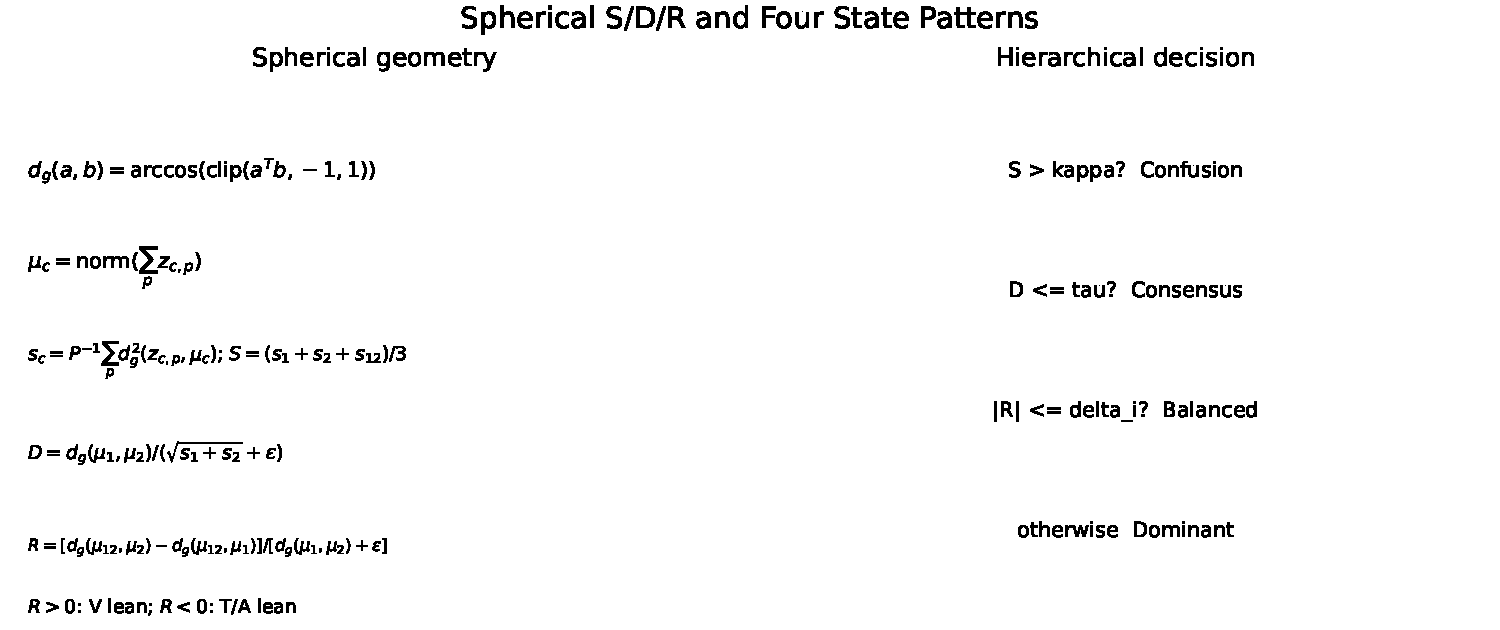
\includegraphics[width=\linewidth]{figures/generated/fig03_spherical_sdr.pdf}
  \caption{Exact spherical S/D/R definitions and hierarchical four-pattern assignment.}
  \label{fig:sdr-method}
\end{figure}

\subsection{Four State Patterns and State-guided Response}

The four patterns are Confusion, Consensus, Balanced, and Dominant.
The same state labels can be used to route a lightweight response policy in Stage 2.

\section{Experiments}

\subsection{Experimental Setup}

This subsection covers datasets, protocols, models, prompt sets, baselines, and metrics.

\subsection{Main Result: Conflict vs Aligned}

This subsection tests whether Conflict and Aligned samples differ in pre-generation state.

\subsection{Main Result: Relation to Wrong Answers}

This subsection tests whether state patterns predict later wrong answers.

\subsection{Baseline Comparison}

Baselines include behavior-only signals, mature uncertainty methods, strong classifiers, and post-hoc full-response analysis.

\subsection{Why \(t_0\): Timing and Efficiency}

This subsection compares pre-generation analysis against full-output post-hoc analysis.

\subsection{Generalization and Case Studies}

This subsection includes one Conflict case, one Aligned case, and one state-guided response case.

\subsection{Limitations and Future Directions}

This subsection records scope limits, including richer protocols, internal temporal information, and broader model panels.

\section{Conclusion}

We study pre-generation misjudgment risk in multimodal affective conflict.
The \(S/D/R\) state analysis makes this risk visible at \(t_0\).
The resulting state patterns provide both interpretability and practical value for downstream response routing.


\bibliographystyle{IEEEtran}
\bibliography{refs}

\end{document}
